\chapter{Pontos Flutuantes}

Na matemática, %os sistemas numéricos são utilizados para representar quantidades por meio de símbolos. 
um sistema numérico é um conjunto de regras e símbolos utilizados para representar quantidades através do que chamamos de números. %que definem como escrevemos e entendemos esses números.
Existem dois tipos de sistemas: os posicionais e os aditivos. 

O sistema aditivo é aquele em que os números são representados pelas somas dos valores dos símbolos, geralmente agrupados lado a lado em ordem decrescente, como, por exemplo, os sistemas romano e egípcio. Já o sistema posicional leva em conta não só os dígitos mas também a posição que eles ocupam no número. %utiliza a posição de cada dígito como múltiplo de uma potência da base. 
%A base de um sistema numérico indica quantos 
A quantidade de símbolos diferentes que são utilizados para representar os dígitos está ligada à \textbf{base} desse sistema, e cada posição do dígito no número refere-se a uma potência dessa base. Por exemplo, no sistema decimal (base 10), usamos os dígitos de 0 a 9. No sistema binário (base 2), usamos os dígitos 0 e 1. E já no sistema hexadecimal (base 16), usamos de 0 a 9 e as letras A a F (que representam 10 a 15).

Com essas diferentes formas de representar um número, a escolha do sistema depende do contexto e da aplicação. No uso cotidiano, a base decimal é a mais utilizada. Já as bases binária e hexadecimal, são amplamente utilizadas na ciência da computação em operações aritméticas dos processadores e em algumas linguagens de programação para endereçamento de memória.

Um número $N$ pode ser representado em uma base \(b\) no seguinte formato
\begin{equation}
N = \pm \sum_{i=-k}^{n} d_i b^i,
\end{equation}
em que \(d_i\) são os dígitos na base \(b\), \(k\) é o número de casas decimais à direita do ponto, e \(n+1+k\) é o número de dígitos significativos. Vejamos alguns exemplos.

\begin{ex}
Vamos escrever o número 13 nas bases 10 e 2.
\begin{itemize}
    \item Número na base decimal: $ 13 = 1 \times 10^1 + 3 \times 10^0 = 13_{10}$
    \item Número na base binária: $ 13 = 1 \times 2^3 + 1 \times 2^2 + 0  \times 2^1 + 1 \times 2^0  = 1101_2$
\end{itemize}
\end{ex}

\begin{ex}
Agora vamos escrever o número 3,5625 nas bases 10 e 2.

\begin{itemize}
    \item Número na base decimal: 
    \[
    3{,}5625 = 3 \times 10^0 + 5 \times 10^{-1} + 6 \times 10^{-2} + 2 \times 10^{-3} + 5 \times 10^{-4} = 3{,}5625_{10}
    \]
    
    \item Número na base binária:
    \[
    3{,}5625 = 1\times 2^{1} + 1 \times 2^0 + 1 \times 2^{-1} + 0 \times 2^{-2} + 0 \times 2^{-3} + 1 \times 2^{-4} = 11{,}1001_2
    \]
\end{itemize}
\end{ex}

\section{Aritmética de Ponto Flutuante}

A \textit{aritmética de ponto flutuante} é o sistema adotado por computadores para que lidem com números reais utilizando uma notação compacta e eficaz. Essa técnica é utilizada para representar e manipular números reais de forma prática e eficiente. Ela permite representar números de grandezas diversas, que não podem ser armazenados com precisão, utilizando apenas números inteiros.


Um sistema de ponto flutuante $F$ pode ser definido como
\[
F(\beta, t, L, U)\]
cuja representação normalizada de um número real N nesse sistema é dada por
\begin{equation}
N = \pm (0.d_{1}d_{2} . . . d_{t})_\beta \times \beta^e 
\end{equation}
em que
\begin{itemize}
  \item \( N \) é o número real;
  \item \(\beta\) é a base que a máquina opera;
  \item \( t \) é o número de dígitos na mantissa, tal que \( 0 \leq d_{j} \leq \beta-1 \), j = 1, ..., t, \(d_{1} \neq 0\);
  \item \( L \) é o menor expoente inteiro;
  \item \( U \) é o maior expoente inteiro;
  \item \( e \) é o expoente inteiro no intervalo [\( L \),\( U \)].
\end{itemize}

%\subsection*{Representação segundo o padrão IEEE 754}

No padrão IEEE 754 (usado na maioria dos sistemas eletrônicos), um número de ponto flutuante é dividido em três partes:

\begin{itemize}
  \item \textbf{Sinal (S)}: 1 bit indicando se o número é positivo (\( S = 0 \)) ou negativo (\( S = 1 \)),
  \item \textbf{Expoente (E)}: campo que representa o expoente com viés (bias),
  \item \textbf{Mantissa (M)}: parte fracionária significativa do número.
\end{itemize}

A fórmula completa de reconstrução do número é:

\[
\text{Valor} = (-1)^S \times (1.M) \times 2^{E - \text{bias}}
\]

onde:

\begin{itemize}
  \item \( S \) é o bit de sinal,
  \item \( 1.M \) indica que há um bit implícito "1" antes da mantissa nos números normalizados,
  \item \( \text{bias} \) é um valor constante que depende da precisão (por exemplo, 127 para 32 bits).
\end{itemize}

\subsection{Precisão Simples e Precisão Dupla}

Em sistemas computacionais, os números em ponto flutuante podem ser representados em diferentes níveis de precisão. Os dois mais comuns são:

\begin{itemize}
  \item \textbf{Precisão Simples (32 bits)}
  \item \textbf{Precisão Dupla (64 bits)}
\end{itemize}

Esses formatos seguem o padrão \texttt{IEEE 754} de representação binária de números reais.

\subsubsection*{Comparação entre os formatos}

\begin{center}
\begin{tabular}{|l|c|c|}
\hline
\textbf{Característica} & \textbf{Precisão Simples (32 bits)} & \textbf{Precisão Dupla (64 bits)} \\
\hline
Bits totais & 32 & 64 \\
\hline
Bit de sinal & 1 & 1 \\
\hline
Bits de expoente & 8 & 11 \\
\hline
Bits de mantissa & 23 & 52 \\
\hline
Bias & 127 & 1023 \\
\hline
Intervalo do expoente real & \(-126\) a \(+127\) & \(-1022\) a \(+1023\) \\
\hline
Precisão (dígitos decimais) & Aproximadamente 7 & Aproximadamente 16 \\
\hline
\end{tabular}
\end{center}

\subsubsection*{Exemplo: Representação em \textbf{Precisão Simples}}

Considere o número decimal \( x = -12{,}25 \). Sua representação em binário é:

\[
x = -1100{,}01_2 = -1{,}10001 \times 2^3
\]

Formato:

\begin{itemize}
  \item Sinal: \( s = 1 \)
  \item Mantissa (sem o bit oculto): \( 10001000000000000000000 \)
  \item Expoente: \( e = 3 + 127 = 130 = 10000010_2 \)
\end{itemize}

Portanto, o número seria representado, em binário de 32 bits, como:

\[
\boxed{1\ 10000010\ 10001000000000000000000}
\]
\subsubsection*{Exemplo: Representação em Precisão Dupla}

Vamos representar o número decimal \( x = 12{,}375 \) em ponto flutuante com \textbf{precisão dupla (64 bits)}.

\paragraph{1. Conversão para binário:}

\[
12{,}375_{10} = 1100{,}011_2 = 1{,}100011 \times 2^3
\]

\paragraph{2. Identificação dos componentes:}

\begin{itemize}
  \item \textbf{Sinal (s)}: Como o número é positivo, \( s = 0 \)
  \item \textbf{Expoente real (e)}: \( 3 \)
  \item \textbf{Bias}: Para precisão dupla, \( \text{bias} = 1023 \)
  \item \textbf{Expoente com bias}: \( e + \text{bias} = 3 + 1023 = 1026 \)
  \item \textbf{Expoente em binário (11 bits)}: \( 1026_{10} = 10000000010_2 \)
  \item \textbf{Mantissa (m)}: Os bits após o ponto da parte fracionária normalizada: \( 100011000000\ldots \) (completando até 52 bits)
\end{itemize}

\paragraph{3. Representação final (64 bits):}

\[
\boxed{
0\ 10000000010\ 1000110000000000000000000000000000000000000000000000
}
\]

\noindent Essa é a representação de \( 12{,}375 \) em ponto flutuante com precisão dupla.

\paragraph{Resumo:}
\begin{itemize}
  \item \textbf{Bits de sinal}: \( 0 \)
  \item \textbf{Bits do expoente}: \( 10000000010 \)
  \item \textbf{Bits da mantissa}: \( 100011 \) seguidos de zeros até completar 52 bits
\end{itemize}


\subsubsection*{Considerações}

A escolha entre precisão simples e dupla depende da aplicação:



\begin{itemize}
  \item \textbf{Precisão Simples}: adequada para aplicações com memória limitada e que não exigem alta precisão.
  \item \textbf{Precisão Dupla}: usada em aplicações científicas, cálculos de engenharia, simulações e algoritmos numéricos mais sensíveis.
Apesar do ganho de precisão, o uso de precisão dupla demanda mais memória e tempo de processamento.


\end{itemize}



\newpage
\subsection{Representação de Números em Sistemas de Ponto Flutuante}

Em máquinas que operam em sistemas de ponto flutuante, apenas um subconjunto finito de \(\mathbb{R} \) pode ser representado de maneira exata. Por isso, frequentemente, é necessário limitar a quantidade de dígitos significativos na representação de números a fim de  adequá-los ao sistema que a máquina opera. Dois dos principais processos empregados para este fim são o \textbf{truncamento} e o \textbf{arredondamento}.

O truncamento consiste na supressão de todos os dígitos após uma determinada posição, sem qualquer ajuste adicional no último dígito mantido. Formalmente, dado um número real \( x \), sua aproximação truncada com \( n \) dígitos na base \( b \) é expressa por
\[
T(x) = \sum_{i = -k}^{n-1} d_i b^i
\]
onde os dígitos \( d_i \) com \( i < -k \) são descartados.

O erro introduzido por este processo, dado por $E_T = x-T(x)$, é denominado \textit{erro de truncamento}. Ele é limitado superiormente por
\begin{equation}
    |x - T(x)| < b^{-k}.
\end{equation}
\begin{ex}
Considere a aproximação com oito casas decimais de \(\pi = 3,14159265\).
Para truncar $\pi$  com precisão de 4 casas decimais, descartamos todos os termos da sexta casa em diante. Assim, o valor truncado fica
$T(\pi) = 3,1415$.
O erro do truncamento é, nesse caso, $E_T = 3,14159265 - 3,1415 = 0,00009265$. Diante disso, podemos observar que $|E_T| < 10^{-4}$.
\end{ex}

O arredondamento, por outro lado, ajusta o último dígito mantido com base no valor do primeiro dígito descartado, buscando minimizar o erro absoluto da aproximação. No arredondamento simétrico (ou clássico), se o primeiro dígito descartado for maior ou igual a \( \frac{b^{-n}}{2} \), incrementa-se o último dígito mantido em uma unidade; caso contrário, seu valor permanece inalterado.

Seja \( x \) um número real e \( R(x) \) sua aproximação arredondada com \( n \) dígitos na base \( b \). O erro de arredondamento satisfaz:

\[
|x - R(x)| \leq \frac{1}{2} b^{-n}
\]

\begin{ex}
Ainda considerando a mesma aproximação de \(\pi = 3,14159265\).
Para arredondar $\pi$  com precisão de 4 casas decimais, vamos analisar o número da próxima casa em que queremos arredondar. Nesse caso, o número na quinta posição é 9, então vamos arredondar para cima. 
$$R(\pi) = 3,1416$$
O erro do arredondamento é, nesse caso, $$E_R = 3,14159265 - 3,1416  = -0,00000735.$$  
Diante disso, podemos observar que $|E_R| \leq  \frac{ 1}{2}10^{-4}$ . %Consequentemente $|E_R| \leq  |E_T|$
\end{ex}

Em geral, o erro máximo introduzido pelo arredondamento é metade daquele introduzido pelo truncamento, razão pela qual o arredondamento tende a produzir aproximações mais precisas.


%\subsection*{Menor e Maior valor num sistema de ponto flutuante}


Para compreendermos melhor as limitações na representação de números em um sistema de ponto flutuante, vamos explorar o exemplo a seguir. Suponha que uma máquina opere no sistema $F(10, 5, -5, 5)$. %{\color{red}
%$F(\beta, t, L ,U)$ em que 
%\[
%\beta = 10; t = 5; L=-5;U=5.
%\]
%}
Nesse sistema, os números serão representados da seguinte maneira
\begin{equation}
\pm (0.d_{1}d_{2} . . . d_{t}) \times 10^e,  0 \leq |d_{j}| \leq 9,  d_{1} \neq 0, e \in [-5,5].
\end{equation}
O menor valor, em módulo, representado nesse sistema é
$$
m = 0.10000 \times 10^{-5} = 10^{-6},
$$
enquanto que o maior é
$$
M = 0.99999 \times 10^{5} = 99999.
$$
O subconjunto $G \subset \mathbb{R}$ definido como
$$
G = \left\{ x \in \mathbb{R} \mid m \leq |x| \leq M \right\}
$$

\[
G = \left\{ x \in \mathbb{R} \mid m \leq |x| \leq M \right\}
\]
é o conjunto dos números que são representáveis por esse sistema de ponto flutuante. Nesse conjunto:
\begin{itemize}
  \item \( m \) é o menor valor positivo representável;
  \item \( M \) é o maior valor representável;
  \item Os números são representados na forma normalizada \( \bar{x} = \pm 0.d_1d_2d_3d_4d_5 \times 10^e \).
\end{itemize}
Dado um número real $x$, as seguintes situações podem ocorrer:

\subsubsection{Caso 1: \( x \in G \) (Número representável)}
Seja $x = 12237,76$. 

Na forma normalizada temos \(x = 0,1223776 \times10^5\).
Porém, esse número não pode ser representado precisamente no sistema $F$ e, portanto, precisamos aplicar uma das técnicas de aproximação. Utilizando o truncamento o resultado é \( \bar{x} = 0{,}12237 \times 10^5 \). Já com o arredondamento \( \bar{x} = 0{,}12238 \times 10^5 \).

O número está dentro da faixa de expoente permitida e é representável com perda controlada de precisão.

\subsubsection*{Caso 2: \( |x| < m \) (Underflow)}

Seja \( x = 0{,}582 \times 10^{-6} \).

O expoente é \(–6\), menor que o limite inferior $L = -5$. Portanto, o número não pode ser representado e ocorre \textbf{underflow}. Nesse caso, na maioria das vezes o valor é tratado como zero.

\subsubsection*{Caso 3: \( |x| > M \) (Overflow)}

Seja \( x = 0{,}927 \times 10^6 \)

O expoente é +6, maior que $U = 5$. 
Portanto, ocorre \textbf{overflow} e o número não pode ser representado precisamente. Neste caso, o valor pode ser tratado como infinito ou como uma flag indicando o \textbf{overflow}.


\subsection{Representação Especial do Zero}

Na representação de ponto flutuante, um número real é geralmente expresso na forma normalizada:

\[
N = \pm (d_1{,}d_2 d_3 \ldots d_t)_\beta \times \beta^{e},
\]
com \( d_1 \neq 0 \), garantindo o aproveitamento máximo da precisão disponível e evitando representações redundantes. Contudo, o número zero não pode ser representado nesta forma, pois exigiria \( d_1 = 0 \), o que contraria a normalização. 

Assim, o zero recebe uma \textit{representação especial} denotada por

\[
N = \pm (0{,}000\ldots 0_{t})_\beta \times \beta^{L - 1},
\]
em que \( L \) é o menor expoente permitido no sistema. Este tratamento especial assegura que o zero seja manipulado de forma única e consistente dentro do sistema de ponto flutuante.

\subsubsection*{Prevenção da perda de significância}

Em operações numéricas envolvendo números de ordens de grandeza muito distintas, pode ocorrer a \textit{perda de significância}, isto é, quando os dígitos significativos de um número pequeno são eliminados na soma ou subtração com um número muito maior.

Considere um sistema de ponto flutuante $F(10, 7, -5, 5)$. Sejam \(
x = 0{,}000 \times 10^{-6} \quad (\text{ou seja, o número zero}), \qquad y = 0{,}276 \times 10^{-2}.
\)

Na operação de soma:

\[
x + y = 0{,}276 \times 10^{-2},
\]

como \( x \) é exatamente zero, o resultado mantém integralmente os dígitos significativos de \( y \).

Se o zero não tivesse uma representação especial e fosse tratado como um subnormal com expoente mínimo, o alinhamento das mantissas poderia comprometer a precisão de \( y \), deslocando seus dígitos significativos e resultando em perda de informação. 

Portanto, a representação especial do zero evita este problema, preservando a precisão e assegurando a estabilidade numérica das operações.

Vejamos a seguir uma comparação da técnicas de arredondamento e de truncamento.

Considere uma máquina decimal com 3 dígitos na mantissa e expoentes variando de –4 a 4:

\begin{center}
\small
\begin{tabular}{|c|c|c|c|c|}
\hline
\textbf{Número Real} & \textbf{Arredondamento} & \textbf{\(E_R\)}  & \textbf{Truncamento} & \textbf{\(E_T\)}  \\
\hline
5{,}678 & \( 0{,}568 \times 10^1 \) & \( 0{,}2 \times 10^{-3} \) & \( 0{,}567 \times 10^1 \) & \( 0{,}8 \times 10^{-3} \) \\
\hline
–192{,}73 & \( -0{,}193 \times 10^3 \) & \( 0{,}27 \times 10^{1} \) & \( -0{,}192 \times 10^3 \) & \( 0{,}73 \times 10^{1} \) \\
\hline
3{,}14159 & \( 0{,}314 \times 10^1 \) & \( 0{,}159 \times 10^{-2} \) & \( 0{,}314 \times 10^1 \) & \( 0{,}159 \times 10^{-2} \) \\
\hline
0{,}0000063 & \multicolumn{4}{c|}{Underflow} \\
\hline
920000{,}0 & \multicolumn{4}{c|}{Overflow} \\
\hline
\end{tabular}
\end{center}

\newpage


\section{Erros e Limitações}

Erros em operações com pontos flutuantes podem se propagar e aumentar em cálculos mais complexos. Por exemplo, pequenos erros de arredondamento em etapas iniciais podem afetar significativamente o resultado final, especialmente em somas repetitivas ou subtrações de números muito próximos. Isso torna importante considerar a ordem das operações e o impacto da precisão em aplicações sensíveis.

\begin{comment}
\subsection{Erro Absoluto e Relativo}

Em cálculos numéricos, frequentemente lidamos com aproximações devido a arredondamentos e truncamentos. Para avaliar a precisão dessas aproximações, utilizamos as métricas de erro absoluto e erro relativo.
  
O erro absoluto mede a diferença entre o valor real \( x_r \) e o valor aproximado \( x_a \), ou seja, a quantidade exata de erro na aproximação. Ele é definido como:

\[
\text{EA} = |x_a - x_r|
\]

Quanto menor for o erro absoluto, mais próxima a aproximação está do valor real. No entanto, essa métrica não fornece informações diretas sobre a importância do erro em relação ao tamanho do número em questão.  

O erro relativo mede o erro absoluto em relação ao valor real, ou seja, indica proporcionalmente o quão distante a aproximação está. Ele é definido como:

\[
\text{ER} = \frac{|x_a - x_r|}{|x_r|}
\]

Essa métrica é útil quando lidamos com valores de grandezas muito diferentes. Por exemplo, um erro absoluto de \( 0.1 \) pode ser insignificante se estivermos tratando de números na ordem de milhares, mas pode ser relevante se estivermos lidando com valores pequenos, como 0.2.  

{Exemplo de Cálculo:} \begin {ex} Considere que temos um valor real \( x_r = 10.5 \) e uma aproximação \( x_a = 10.3 \). Podemos calcular os erros conforme segue:

\begin{itemize}
    \item \textbf{Erro absoluto:}  
    \[
    |10.3 - 10.5| = 0.2
    \]
    \item \textbf{Erro relativo:}  
    \[
    \frac{0.2}{10.5} \approx 0.019
    \]
\end{itemize}

Neste caso, o erro absoluto é \( 0.2 \), o que indica que nossa aproximação difere do valor real por essa quantidade. O erro relativo, sendo aproximadamente \( 0.019 \) (ou 1.9\%), nos mostra que essa diferença representa menos de 2\% do valor real, indicando que a aproximação é razoavelmente precisa.
\end {ex}

O erro relativo se torna crucial quando lidamos com números muito grandes ou muito pequenos. Por exemplo:

\begin{itemize}
    \item Se tivermos um valor real de \( 10^6 \) e um erro absoluto de \( 1 \), isso representa um erro relativo extremamente pequeno (\( 10^{-6} \)), indicando que a aproximação é muito boa.
    \item Se tivermos um valor real de \( 0.0005 \) e um erro absoluto de \( 0.0001 \), o erro relativo será \(\frac{0.0001}{0.0005} = 0.2\), ou seja, 20\%, um valor bastante alto, indicando uma aproximação ruim.
\end{itemize}

Portanto, o erro relativo nos ajuda a interpretar melhor a qualidade de uma aproximação, independentemente da escala dos números envolvidos.

\end{comment}


\section{Perda de Significância em Somas}
A perda de significância (também conhecida como cancelamento catastrófico) ocorre de modo mais severo quando há grande diferença de ordem de grandeza entre os números envolvidos na operação. Por exemplo, considere:

\[
x = 1{,}000 \times 10^{4} \quad \text{e} \quad y = 0{,}276 \times 10^{-2}.
\]

Para realizar a soma, ambos os operandos precisam ser expressos com o mesmo expoente:

\[
x = 1{,}000000000 \times 10^4, \quad y = 0{,}000000276 \times 10^4.
\]

A soma exata seria:

\[
x + y = (1{,}000000000 + 0{,}000000276) \times 10^4 = 1{,}000000276 \times 10^4.
\]

Contudo, devido à precisão limitada do sistema (7 dígitos significativos), a aritmética de ponto flutuante armazena apenas:

\[
x + y \approx 1{,}0000002 \times 10^4.
\]

Uma parte do termo \( y \) é completamente desprezada, e a soma não resulta numericamente igual a \( x + y\), evidenciando a perda catastrófica de significância.

Outro caso peculiar é a soma de um número muito grande com uma sequência de números pequenos. Dependendo da ordem em que as somas são realizadas, o número grande pode "mascarar" os pequenos, resultando em diferentes valores finais.

Por exemplo:
\[
S = 10^{8} + 10^{-1} + 10^{-2} + 10^{-3} + \ldots + 10^{-10}.
\]
Se somarmos primeiro o número grande (\(10^8\)) e depois os números pequenos, muitos destes podem ser ignorados devido à falta de precisão da mantissa. Por outro lado, ao somar os números pequenos antes, o valor final será mais próximo do esperado.

Para ilustrar, suponha a seguinte ordem de cálculo:
\begin{itemize}
    \item Caso 1: \(S = 10^{8} + (10^{-1} + 10^{-2} + \ldots + 10^{-10})\).
    \item Caso 2: \(S = (10^{-1} + 10^{-2} + \ldots + 10^{-10}) + 10^{8}\).
\end{itemize}
No primeiro caso, muitos números pequenos são ignorados devido ao arredondamento. No segundo, o somatório dos números pequenos é calculado antes de adicionar o número grande, preservando mais informações significativas.

\subsection{Análise de Instabilidades e Casos Peculiares}

Na aritmética de ponto flutuante, certos casos resultam em erros devido à limitação da precisão e à maneira como os números são representados. A seguir, descrevemos dois exemplos clássicos que ilustram essas instabilidades.

\subsubsection{Imprecisão de operações de Ponto flutuante}
Considere o cálculo de $f(x) = x^{10} + 1 - x^{10}$ para \(x \in [-60, 60]\). As partes envolvendo $x$ são variáveis e a parte "$1$" é o literal, ou seja, um valor fixo. Analiticamente, o resultado deveria ser exatamente 1. No entanto, em implementações numéricas, pequenas imprecisões na representação de \(x^{10}\) podem levar a resultados instáveis, especialmente para valores de \(|x|\) além de um limiar. Isso ocorre devido ao erro relacionado às operações de ponto flutuante, como mostrado na Figura \ref{fig:catastrofic_cancelation}. 

\begin{figure}[h]
    \centering 
    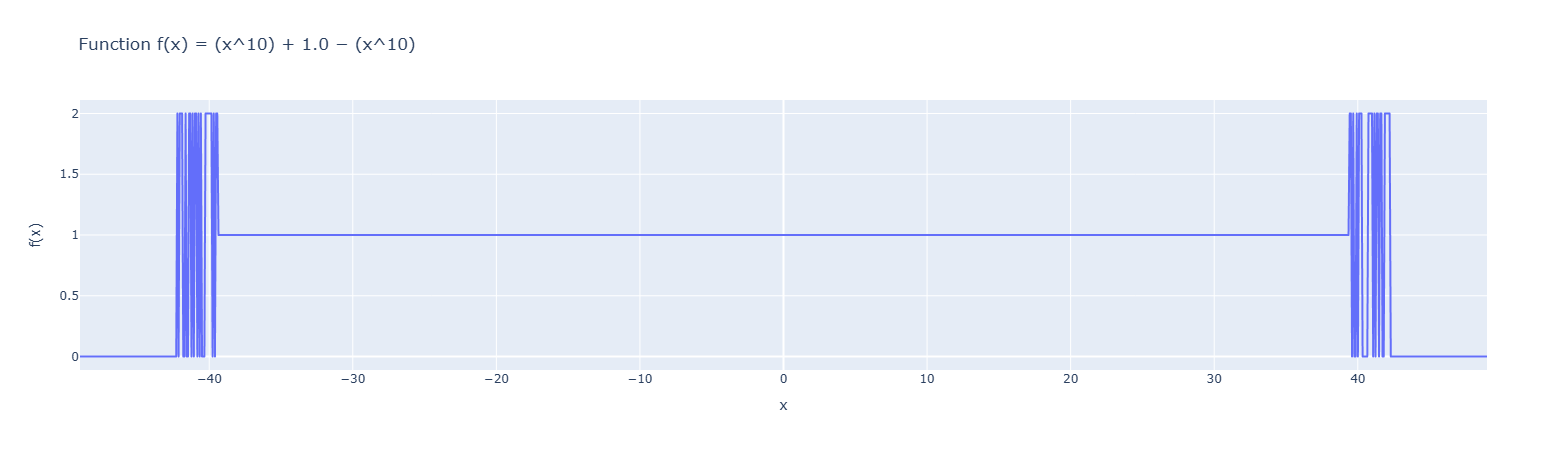
\includegraphics[width=1\textwidth]{Imagens/catastrofic_cancelation.png}
    \caption{Comportamento da expressão \(x^{10} + 1 - x^{10}\) no intervalo \([-40, 40]\).}
    \label{fig:catastrofic_cancelation}
\end{figure}
\begin{figure}[h]
    \centering 
    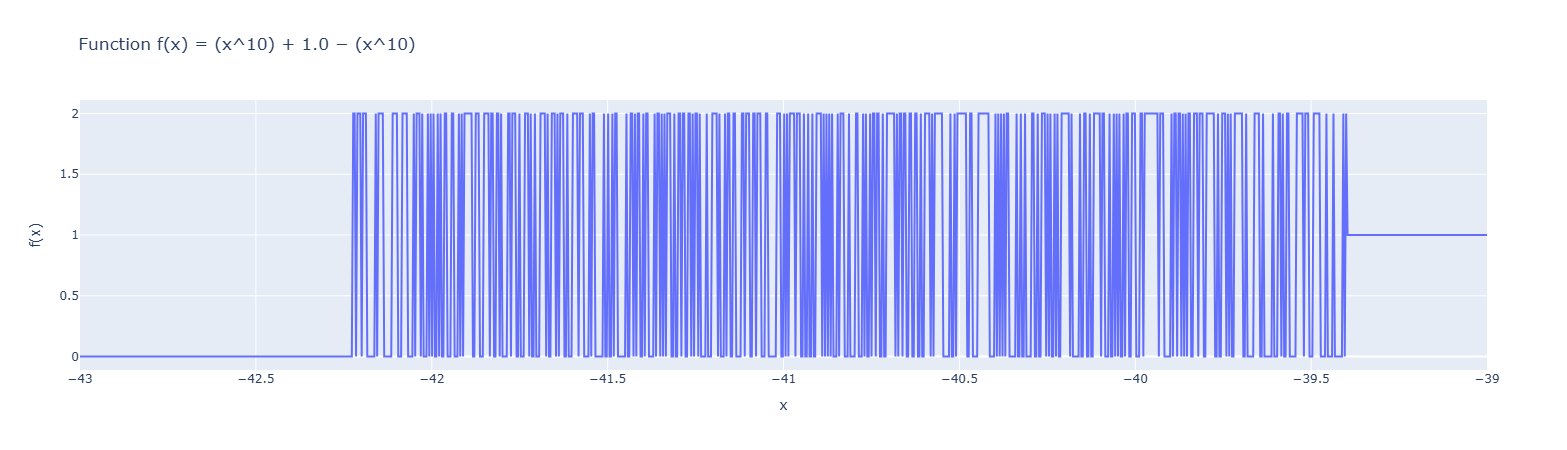
\includegraphics[width=1\textwidth]{Imagens/zoom.png}
    \caption{Comportamento da expressão \(x^{10} + 1 - x^{10}\) no intervalo \([-43, -39]\).}
    \label{fig:zoom}
\end{figure}

Podemos observar que em um determinado limiar, a função para de se comportar como esperado $f(x) = 1$ e passa a assumir valores os de  $f(x) = 2$ e $f(x) = 0$.

Vamos manipular essa expressão e ver como ela se comporta em diferentes situações.

\begin{figure}[h]
    \centering 
    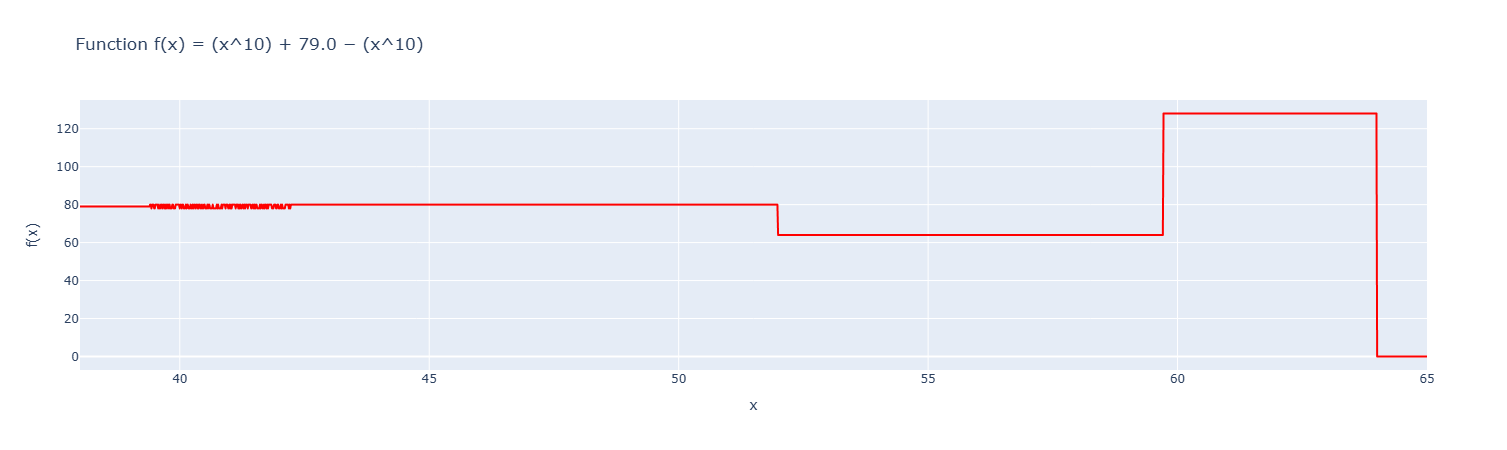
\includegraphics[width=1\textwidth]{Imagens/literal79.png}
    \caption{Comportamento da expressão \(x^{10} + 79 - x^{10}\) no intervalo \([40, 65]\).}
    \label{fig:literal79}
\end{figure}

Na figura  \ref{fig:literal79}. é possível observar que a função assume mais de dois valores inesperados para $f(x)$, nesse caso, o conjunto imagem no intervalo \([40, 65]\) é \( Im(f)  = \bigl\{ {0{,}64{,}78{,}79{,}80{,}128}\}\). Em geral, para literais múltiplos de 3, a função assume 3 ou mais valores inesperados.

Explicação: blablabla

Uma dúvida comum é se a precisão desses sistemas afeta nessa expressão. Vamos comparar então um sistema de float32 (Cerca de 7-8 bits dígitos decimais de precisão) a um sistema float64
(Cerca de 15-16  dígitos decimais de precisão)
\begin{figure}[h]
    \centering 
    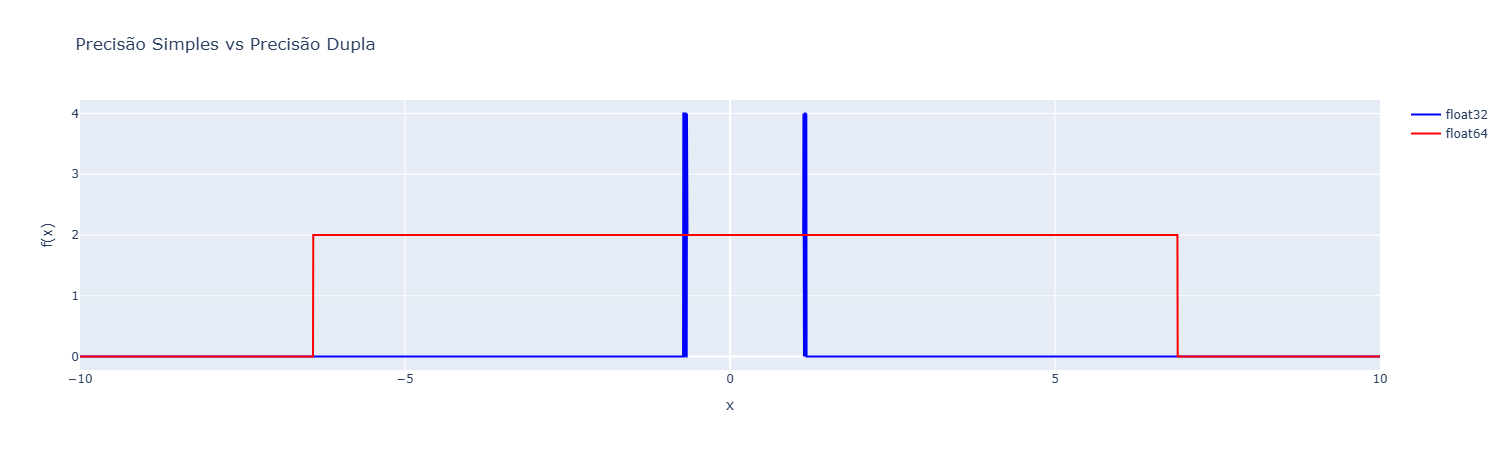
\includegraphics[width=1\textwidth]{Imagens/32x64_full.png}
    \caption{Comportamento da expressão \(x^{10} + 2 - x^{10}\) no intervalo \([10, 10]\).}
    \label{fig:32x64_full}
\end{figure}

\begin{figure}[h]
    \centering 
    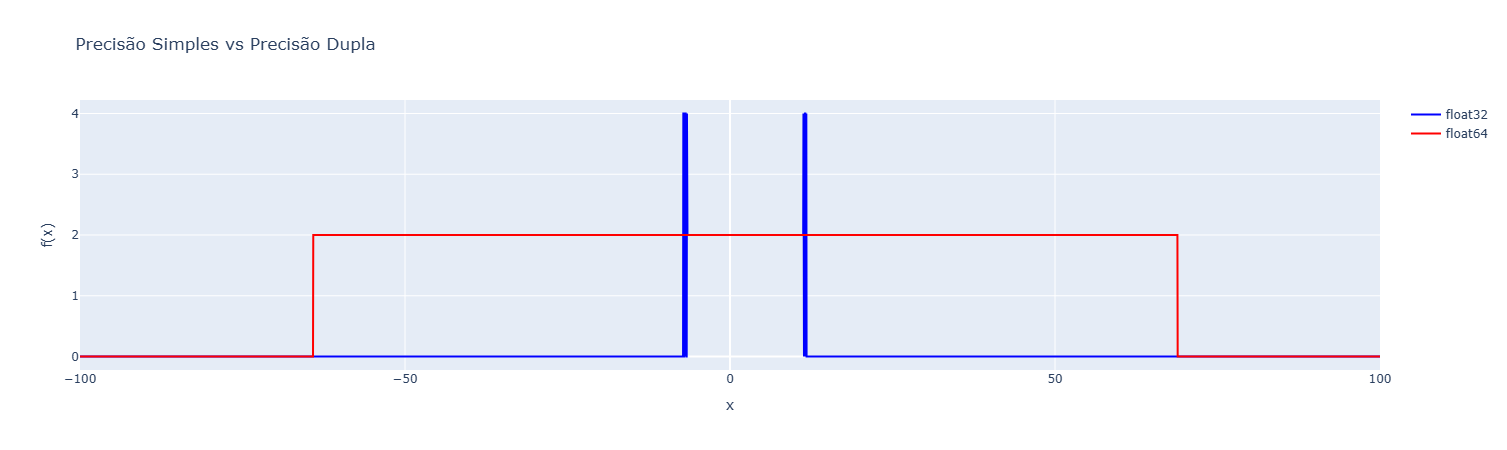
\includegraphics[width=1\textwidth]{Imagens/32x64_full_2.png}
    \caption{Comportamento da expressão \(x^{10} + 2 - x^{10}\) no intervalo \([100, 100]\).}
    \label{fig:32x64_full_2}
\end{figure}

Podemos observar em \ref{fig:32x64_full} e \ref{fig:32x64_full_2} que a função mantém o mesmo comportamento em intervalos diferentes.
Explicação: ?????

\begin{figure}[h]
    \centering 
    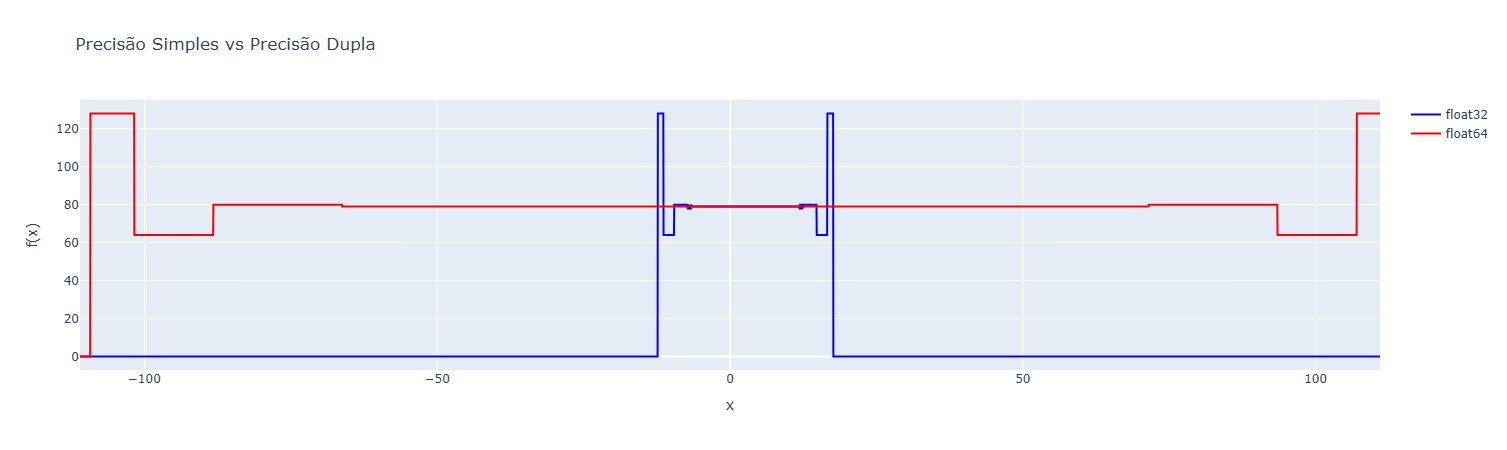
\includegraphics[width=1\textwidth]{Imagens/32x64_full_diffent_extrems.png}
    \caption{Comportamento da expressão \(x^{10} + 79 - x^{10}\) no intervalo \([100, 100]\).}
    \label{fig:32x64_full_diffent_extrems}
\end{figure}

Em \ref{fig:32x64_full_diffent_extrems} a Função se comporta diferente nos 2 extremos.
Explicação: ?????

\begin{figure}[h]
    \centering 
    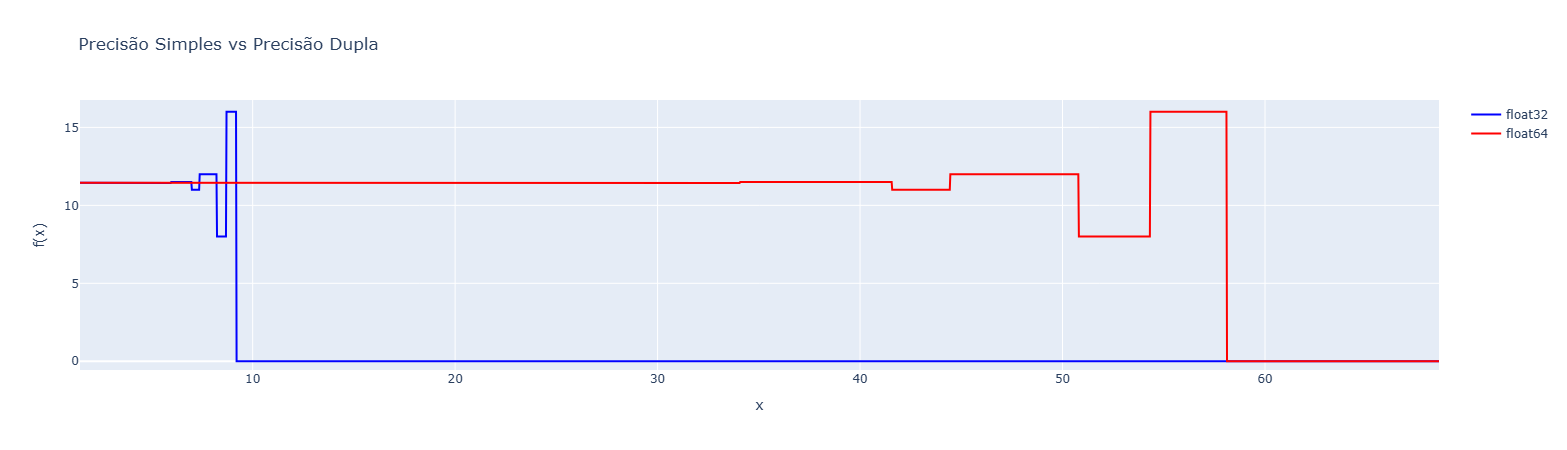
\includegraphics[width=1\textwidth]{Imagens/32x64.png}
    \caption{Comportamento da expressão \(x^{10} + 11.444342323244 - x^{10}\) no intervalo \([0, 60]\).}
    \label{fig:32x64}
\end{figure}

Em geral, como mostrado nas figuras \ref{fig:32x64_full}, \ref{fig:32x64_full_2}, \ref{fig:32x64_full_diffent_extrems} e \ref{fig:32x64} que a instabilidade ocorre onde o $|x|$ da precisão simples é menor do que na precisão dupla.

Outro caso interessante é quando analisamos a função $f(x) = (x\times x\times x\times x\times x\times x\times x\times x \times x) - x^{10} $. Vejamos o gráfico dessa função.
\begin{figure}[H]
    \centering 
    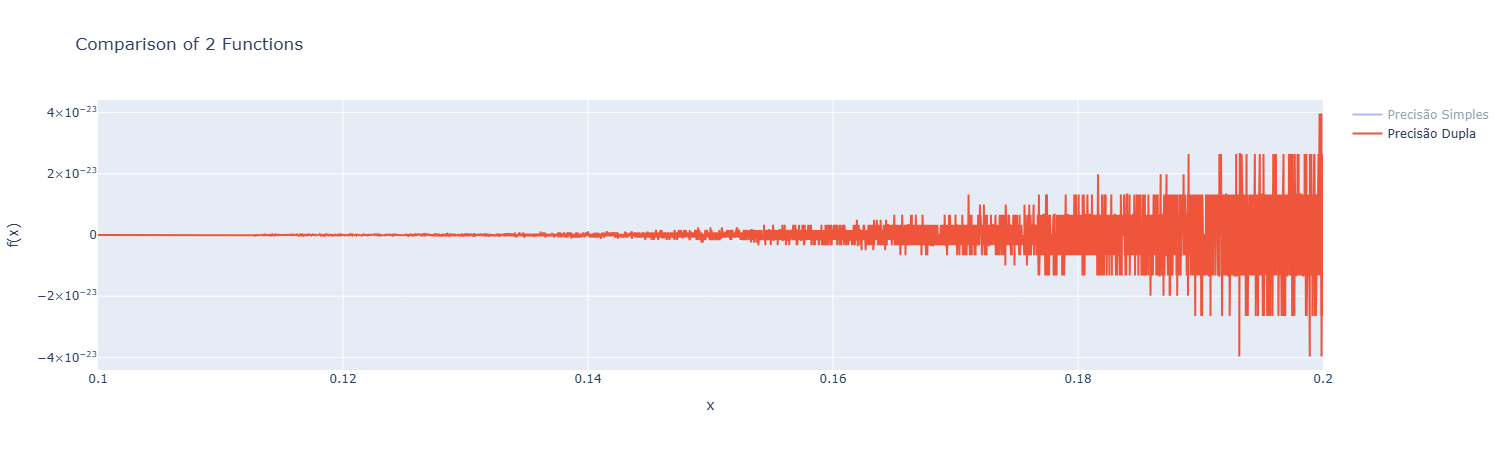
\includegraphics[width=1\textwidth]{Imagens/timesXpot_literal0.png}
    \caption{Comportamento da expressão $f(x) = (x \times x \times x \times x \times x \times x \times x \times x \times x) - x^{10}$, com precisão dupla, no intervalo \([0{,}1, 0{,}2]\).}
    \label{fig:timesXpot_literal0}
\end{figure}

\begin{figure}[H]
    \centering 
    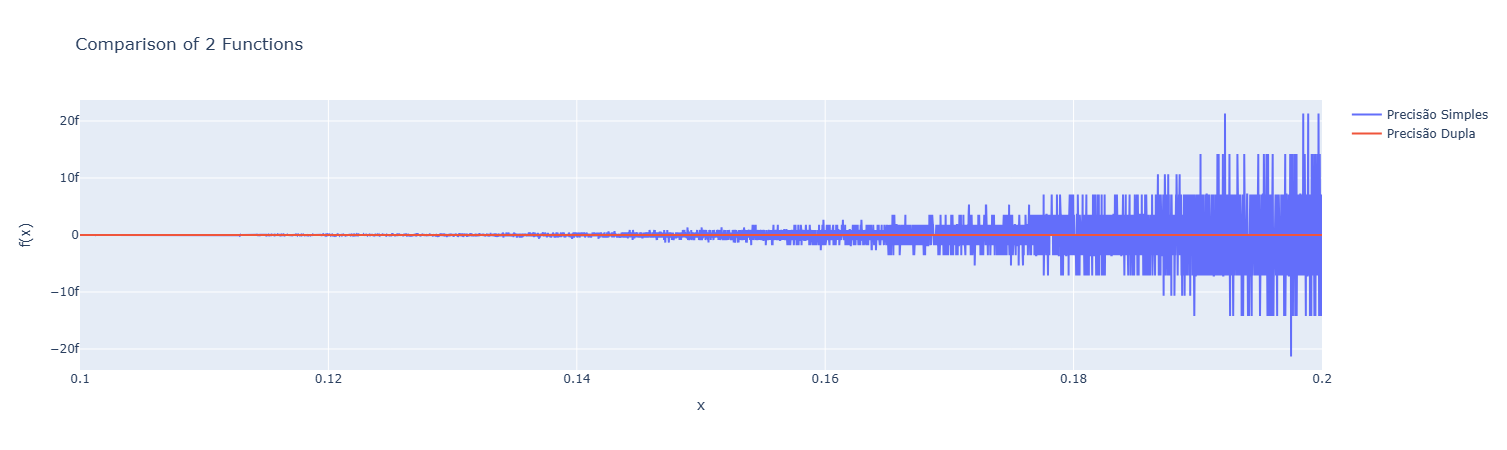
\includegraphics[width=1\textwidth]{Imagens/timesXpot_literal0_1.png}
    \caption{Comportamento da expressão $f(x) = (x \times x \times x \times x \times x \times x \times x \times x \times x) - x^{10}$, com precisão simples, no intervalo \([0{,}1, 0{,}2]\).}
    \label{fig:timesXpot_literal0_1}
\end{figure}

A instabilidade na precisão simples (Figura~\ref{fig:timesXpot_literal0_1}) ocorre em torno de $2 \times 10^{-23}$, enquanto na precisão dupla (Figura~\ref{fig:timesXpot_literal0}) está em torno de $10^{-15}$ (10 femto). Observa-se, portanto, que a diferença de instabilidade é extremamente menor na precisão dupla em comparação com a simples.

Uma outra situação é a diferença de como o computador interpreta algumas funções se forem reescritas de maneiras diferentes. Seja $p(x) = (x - 1)^6$ e $q(x) = x^6 - 6x^5 + 15x^4 - 20x^3 + 15x^2 - 6x + 1$, analiticamente essas funções são idênticas, porém existem problemas de cancelamento catastrófico na hora de analisarmos ambas em um sistema de ponto flutuante.

\begin{figure}[H]
    \centering 
    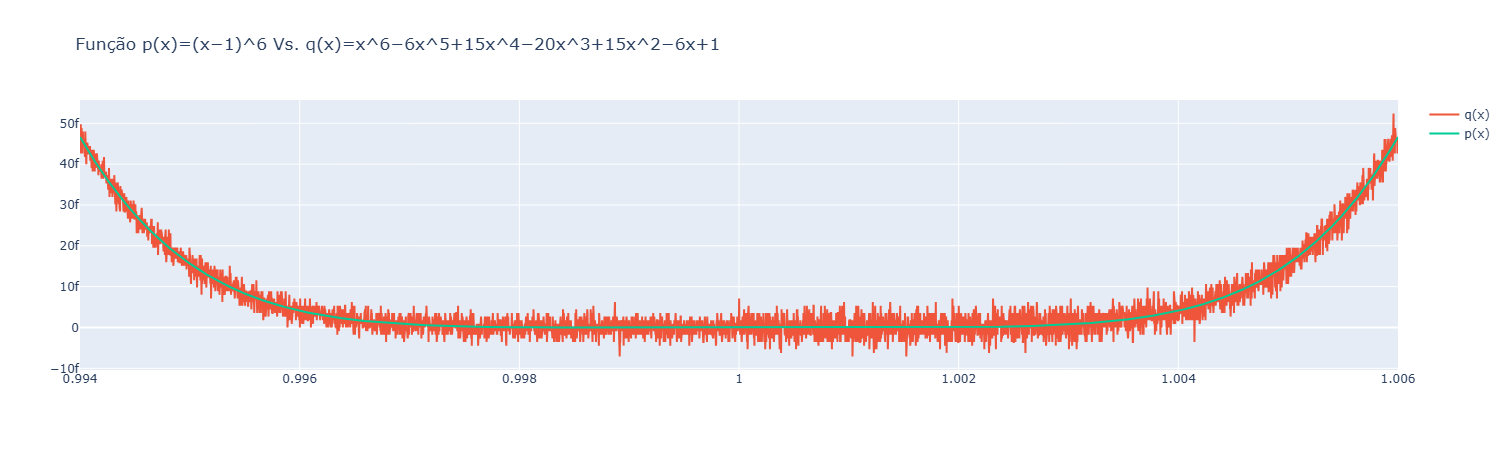
\includegraphics[width=1\textwidth]{Imagens/error2.png}
    \caption{Comparação entre as funções $p(x) = (x - 1)^6$ e $q(x) = x^6 - 6x^5 + 15x^4 - 20x^3 + 15x^2 - 6x + 1$.}
    \label{fig:error2}
\end{figure}
Explicação: yada yada yada 

\subsection{Discussão}

Esses exemplos destacam a importância da ordem das operações e da análise cuidadosa ao trabalhar com algoritmos numéricos. Técnicas como a reordenação de cálculos e o uso de formatos de precisão estendida podem ajudar a minimizar esses erros em contextos críticos.
